\definecolor{srblue}{RGB}{196,124,73}
\definecolor{srgreenfill}{RGB}{255,244,232}
\definecolor{srgreendraw}{RGB}{198,132,76}
\definecolor{srorangefill}{RGB}{255,236,214}
\definecolor{srorangedraw}{RGB}{221,132,59}
\definecolor{srgrayfill}{RGB}{252,245,238}
\definecolor{srgraydraw}{RGB}{141,118,100}
\definecolor{srtext}{RGB}{34,38,45}

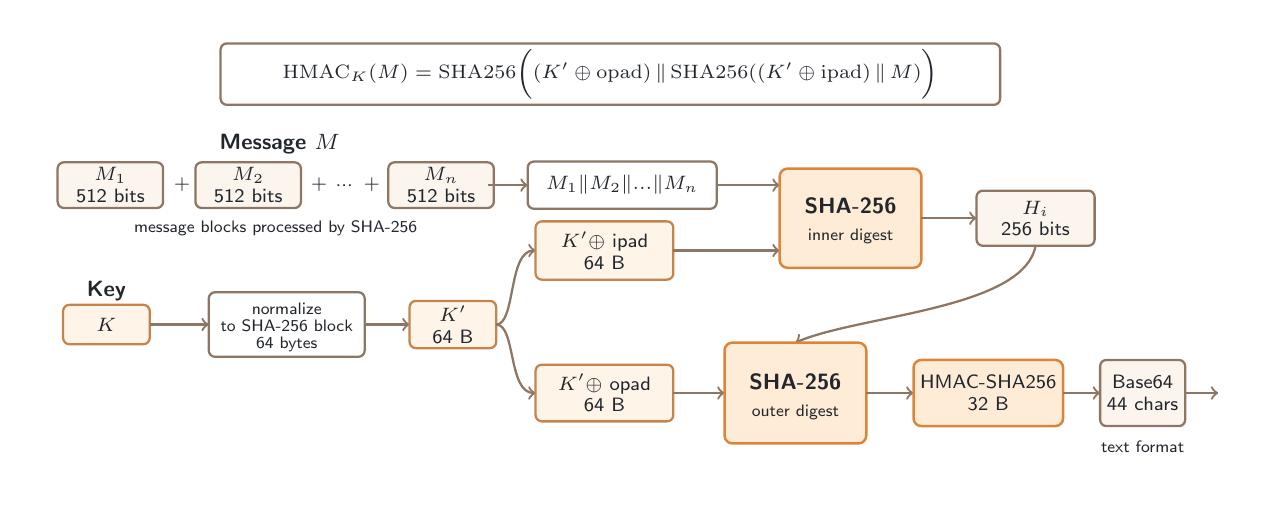
\begin{tikzpicture}[
  x=1cm,
  y=1cm,
  every node/.style={inner sep=0pt, outer sep=0pt},
  label/.style={font=\sffamily\fontsize{7.2}{7.8}\selectfont, text=srtext, align=center},
  smalllabel/.style={font=\sffamily\fontsize{6.4}{7.0}\selectfont, text=srtext, align=center},
  title/.style={font=\sffamily\bfseries\fontsize{7.8}{8.4}\selectfont, text=srtext, align=center},
  formula/.style={font=\sffamily\fontsize{7.0}{7.6}\selectfont, text=srtext, align=center},
  block/.style={draw=srgraydraw, fill=srgrayfill, rounded corners=0.08cm, line width=0.82pt},
  keybox/.style={draw=srgreendraw, fill=srgreenfill, rounded corners=0.08cm, line width=0.82pt},
  hmacbox/.style={draw=srorangedraw, fill=srorangefill, rounded corners=0.10cm, line width=0.9pt},
  opbox/.style={draw=srgraydraw, fill=white, rounded corners=0.08cm, line width=0.82pt},
  flow/.style={draw=srgraydraw, line width=0.82pt, ->}
]

  \path[use as bounding box] (0,0) rectangle (15.35,6.05);

  \begin{scope}[yshift=-0.15cm]

  % Formula inspired by the MAC/HMAC notation used in the course slides.
  \draw[opbox] (2.45,5.22) rectangle (12.35,6.00);
  \node[formula] at (7.40,5.61)
    {\(\mathrm{HMAC}_{K}(M)=\mathrm{SHA256}\big((K' \oplus \mathrm{opad}) \,\Vert\, \mathrm{SHA256}((K' \oplus \mathrm{ipad}) \,\Vert\, M)\big)\)};

  % Message split into SHA-256 input blocks.
  \node[title] at (3.20,4.72) {Message \(M\)};
  \draw[block] (0.38,3.91) rectangle (1.72,4.49);
  \node[label] at (1.05,4.20) {\(M_1\)\\512 bits};
  \node[label] at (1.96,4.20) {+};
  \draw[block] (2.13,3.91) rectangle (3.47,4.49);
  \node[label] at (2.80,4.20) {\(M_2\)\\512 bits};
  \node[label] at (3.70,4.20) {+};
  \node[label] at (4.02,4.20) {...};
  \node[label] at (4.37,4.20) {+};
  \draw[block] (4.58,3.91) rectangle (5.92,4.49);
  \node[label] at (5.25,4.20) {\(M_n\)\\512 bits};
  \node[smalllabel] at (3.15,3.65) {message blocks processed by SHA-256};

  % Key normalization.
  \node[title] at (1.00,2.85) {Key};
  \draw[keybox] (0.45,2.18) rectangle (1.55,2.68);
  \node[label] at (1.00,2.43) {\(K\)};
  \draw[flow] (1.55,2.43) -- (2.30,2.43);
  \draw[opbox] (2.30,2.02) rectangle (4.28,2.84);
  \node[smalllabel] at (3.29,2.63) {normalize};
  \node[smalllabel] at (3.29,2.41) {to SHA-256 block};
  \node[smalllabel] at (3.29,2.18) {64 bytes};
  \draw[flow] (4.28,2.43) -- (4.85,2.43);
  \draw[keybox] (4.85,2.13) rectangle (5.95,2.73);
  \node[label] at (5.40,2.43) {\(K'\)\\64 B};

  % Inner branch.
  \draw[flow] (5.95,2.43) .. controls (6.20,2.43) and (6.10,3.37) .. (6.45,3.37);
  \draw[keybox] (6.45,3.00) rectangle (8.20,3.74);
  \node[label] at (7.325,3.37) {\(K' \oplus\) ipad\\64 B};
  \draw[flow] (5.85,4.20) -- (6.35,4.20);
  \draw[opbox] (6.35,3.90) rectangle (8.75,4.50);
  \node[label] at (7.55,4.20) {\(M_1 \Vert M_2 \Vert ... \Vert M_n\)};
  \draw[flow] (8.20,3.37) -- (9.55,3.37);
  \draw[flow] (8.75,4.20) -- (9.55,4.20);
  \draw[hmacbox] (9.55,3.15) rectangle (11.35,4.41);
  \node[title] at (10.45,3.94) {SHA-256};
  \node[smalllabel] at (10.45,3.55) {inner digest};
  \draw[flow] (11.35,3.78) -- (12.05,3.78);
  \draw[block] (12.05,3.43) rectangle (13.55,4.13);
  \node[label] at (12.80,3.78) {\(H_i\)\\256 bits};

  % Outer branch.
  \draw[flow] (5.95,2.43) .. controls (6.20,2.43) and (6.10,1.56) .. (6.45,1.56);
  \draw[keybox] (6.45,1.20) rectangle (8.20,1.92);
  \node[label] at (7.325,1.56) {\(K' \oplus\) opad\\64 B};
  \draw[flow] (12.80,3.43) .. controls (12.65,2.62) and (10.55,2.55) .. (9.75,2.20);
  \draw[flow] (8.20,1.56) -- (8.85,1.56);
  \draw[hmacbox] (8.85,0.92) rectangle (10.65,2.20);
  \node[title] at (9.75,1.70) {SHA-256};
  \node[smalllabel] at (9.75,1.31) {outer digest};
  \draw[flow] (10.65,1.56) -- (11.25,1.56);
  \draw[hmacbox] (11.25,1.14) rectangle (13.15,1.98);
  \node[label] at (12.20,1.56) {HMAC-SHA256\\32 B};
  \draw[flow] (13.15,1.56) -- (13.62,1.56);
  \draw[block] (13.62,1.14) rectangle (14.70,1.98);
  \node[label] at (14.16,1.56) {Base64\\44 chars};
  \draw[flow] (14.70,1.56) -- (15.12,1.56);

  \node[smalllabel] at (14.16,0.88) {text format};

  \end{scope}

\end{tikzpicture}
